\chapter{Design-ul aplicației server}
\section{Introducere}
\par \textbf{În acest capitol, în secțiunea 5.2, se stabilesc funcțiile serverului și se prezintă tehnologiile folosite la producerea aplicației server. În secțiunea 5.3 se explică mecanismul adoptat pentru atingerea unui scop important, ”scalabilitatea aplicației” . În secțiunea 5.4 se stabilește modul și formatul de reprezentare a datelor transmise între aplicația client și aplicația server. Secțiunea 5.5 este dedicată prezentării părții celei mai relevante din diagrama claselor. În secțiunea 5.6 sunt stabiliți parametrii testului privind scalabilitatea aplicației, codificarea testului și rezultatele fiind expuse în Anexa B. Testul modului de comunicare și a eficienței comunicării intre client și server s-a efectuat pentru capitolul anterior, rezutatele fiind publicate în Anexa A. } 

\section{Funcțiile aplicației server}
\subsection{Funcții de bază ale serverului} 
\begin{itemize}
\item Asigurarea comunicării înspre una sau mai mule aplicații client.
\item Asigurarea comunicării între clienți prin intermediul serverului.
\item Stocarea datelor referitoare la activitățile întreprinse de către utilizatori într-o bază de date.
\item Eliberarea datelor din baza de date, la cererea utilizatorului.
\item Stocarea și publicarea informațiilor ce descriu geometria lumii virtuale.
\item Stocarea și publicarea acțiunilor utilizatorilor ce au efect asupra limii virtuale.
\end{itemize}

\par Serverul are scop demonstrativ. Funcția de securitate a datelor la transfer și la stocare este ignorată. De asemenea, implementarea funcțiilor se realizează in cel mai simplu mod posibil, pentru reducerea complexității și dimensiunii aplicației.

\subsection{Aspecte tehnice și principii generale de design}
\subsubsection{Limbaje de programare}
\par Codificarea aplicției server se va executa în limbajele de programare Java și JavaScript.
\par Java este probabil cel mai potrivit limbaj pentru implementarea aplicațiilor server datorită numărului mare de  biblioteci software utilizate pentru realizarea schimbului de date în rețelele de calculatoare. Acestea pun la dispoziția programatorului o multitudine de funcții de nivel înalt pentru comunicarea la distanță folosind diverse protocoale de comunicație de nivel înalt (HTTP/FTP/SSH/etc), cât și funncții de nivel mediu (bazate pe protocoalele TCP/UDP/etc..). Implementarea unei aplicații scalabile prin utilizarea ”plug-in”-urlior este relativ usor de realizat. Existența unui interpretor JavaScript pentru platforma Java este încă un argument în favoarea folosirii acestui limbaj de programare.
\subsubsection {Sistemul de operare}
\par Aplicațiile java sunt extrem de portabile, acestea rulând pe virtual orice sistem de operare și pe orice platformă hardware. Serverul mediului de învățare 3D va rula în varianta pentru GNU/Linux a ”Mașinii Virtuale Java” (JVM). Fiabilitatea kernelului sistemului de operare Linux va afecta pozitiv viteza de rulare a mașinii virtuale java cu efect direct asupra performanței aplicației server dezvoltate pentru mediul virtual 3D.
\subsubsection{Principii generale de design}
\par \textbf{Pentru intermedierea comunicării între utilizatori} sau pentru orice fel de notificări trimise utilizatorilor s-a ales un tipar cunoscut în domeniul informatic sub numele ”Observer Pattern”. Această metodă definește și utilizează o dependență 1 → n între obiecte astfel încât un obiect își modifică starea, toate obiectele dependente sunt notificate. Aplicat, în cazul serverului (1) , când un set de date este prelucrat, utilizatorii (n) sunt notificați.
\par \textbf{Pentru a realiza o aplicație scalabilă} se utilizează mecanismul de extindere dinamică a fincționalității cu ”plug-in”-uri. 
\section{Mecanism pentru obținera \\ scalabilității aplicației server}

\par Se va urmări o cît mai mare flexibilizare a sistemului, astfel încât dezvoltarea ulterioară sa fie cât mai facilă. Pentru realizarea acestui obiectiv se va urmări integrarea limbajului de scriptare JavaScript, în serverul sistemului. Se are în vedere folosirea mecanismului de extindere dinamică a funcționalității sistemului prin ”plug-in”-uri. 
\par Utilizatorul, prin intermediul programului client al mediului virtual 3D, expediază \textbf{comenzi} și \textbf{informații} către server cu \textbf{scopul} de a fi prelucrate de către server și returnate sub forma de comezi ce urmează a fi executate de către aplicația client, cu \textbf{efecte} asupra reprezentării mediului virtual 3D.

\begin{center}
\rule{150mm}{.1pt}
\end{center}

\par \textbf{DEF:} \textit{Un} \textbf{plug-in} \ref{fig:imag35} \textit{este o componentă software care poate fi integrată de către aplicația gazdă la momentul execuției sau imediat la începutul procesului de execuție. De cele mai multe ori ”plug-in”-urile sunt salvate în formă binară.}

\begin{figure}[h]
    \centering
    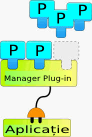
\includegraphics[]{PLA}
    \caption{Arhitectura Plug-in}
    \label{fig:imag35}
\end{figure}

\begin{center}
\rule{150mm}{.1pt}
\end{center}

\subsection{Interfața PLUG-IN-ului}
\par ”Plug-in”-urile aplicației server implementează următoarea interfață:
\begin{verbatim}
public interface CommandTypeDependentInterpreter {
      
      public static final int XML_FORMAT = 1;
      public static final int PALIN_TEXT_FORMAT = 2;
      public void prepareResponse(ServerCommand execCmd, int format);
      String getInterpretedResult();

}
\end{verbatim}

Un plug-in extinde funcționalitatea aplicației server prin introducerea unei noi modalități prin care serverul răspunde la o cerere din partea aplicației client. În prima etapă, plug-in-ul preia comanda expediată de aplicația client prin intermediul metodei: \begin{center} \textit{-- prepareResponse(ServerCommand execCmd, int format) --}
\end{center} În a doua etapă, rezultatul interpretării și procesării datelor de către plug-in se va returna în vederea expedierii către utilizator.

\subsection{Tipuri de plug-in-uri dezvoltate pentru serverul mediului de învățare 3D}
\par Două \textbf{tipuri de plug-in-uri} au fost dezvoltate pentru aplicația server. Primul tip de plug-in este \textbf{”clasic”}, implementat folosind 100\% limbajul Java. Al doilea tip de plug-in este \textbf{”hibrid”}. La inplementarea acestuia sunt utilizate două libmaje de programare: \textbf{Java și JavaScript}. Aces tip de plug-in este o noutate.

\par În principiu, un plug-in hibrid are rolul de a executa la nivelul serverului instrucțiuni codificate în limbaj JavaScript în numele aplicației client. Rezultatele sunt încapsulate în format XML și sunt returnate programului client pentru interpretere. Executarea comenzilor primite de la aplicația client este precedată de următorii doi pași pregătitori: inițializarea unui motor de prelucrare JavaScript ( clasa ScriptEngineManager ) și concatenera la comanda utilizatorului a unei biblioteci care conține obiecte JavaScript utile.\\

\begin{figure}[h]
    \centering
    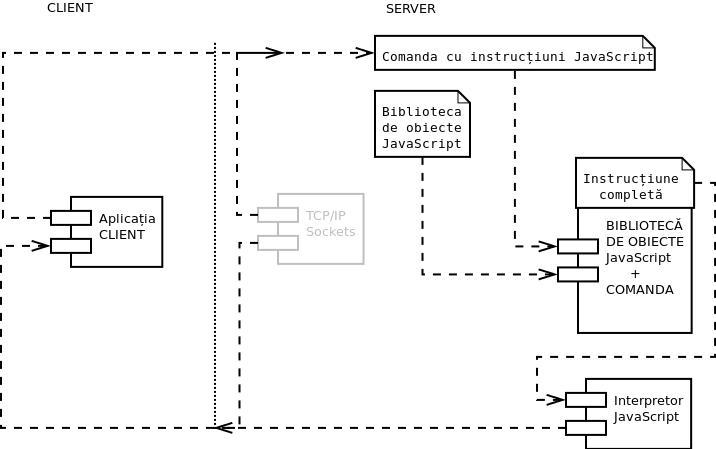
\includegraphics[scale=0.5]{plug-in-js}
    \caption{Schema Plug-in Hibrid}
    \label{fig:imag6}
\end{figure}

\pagebreak

\par Avantajele plug-in-urilor hibride:
\begin{itemize}
\item Se pot descrie și implementa mult mai ușor și mai rapid.
\item Bibloteca de obiecte JavaScript se concatenează la fiecare comandă trimisă de utilizator. Astfel, orice utilizator poate beneficia de obiectele conținute de această bibliotecă de obiecte.
\item Codul se execută la nivelul seerverului, cu efect în creșterea vitezei de lucru a programului client.
\end{itemize}

\par Dezavantajele plug-in-urilor hibride:
\begin{itemize}
\item Comenzile JavaScript invalide pot destabiliza aplicația server.
\item Codul se execută la nivelul serverului, cu efect în descreșterea vitezei de lucru a acestuia.
\item Folosirea limbajului JavaScript introduce diverse riscuri de securitate a datelor.
\end{itemize}



\subsection{Descrierea mecanismului de încărcare a plug-in-urilor}

\par Serverul va ține evidența plugin-urilor disponibile într-un fișier de configurare, organizat în format XML.
\begin{verbatim}
<?xml version="1.0" encoding="UTF-8"?>
<!-- numele comenzii trimise de client -->
<!-- tipul comenzii (CLASIFICARE) -->
<!-- text ajutător (documentatie) -->
<!-- numărul paramerilor .. si expersia (reg-exp) pt diverse prelucrari -->
<!-- plug-in client delegat sa execute acțiuni în aplicația client -->
<!-- sursa de unde poate fi descărcat ălug-in-ul client -->
<!-- executorul .. este plug-in-ul in aplicația server delegat pentru procesarea datelor peimite -->
<!-- .. de la utilizator (CLIENT) -->
<commands>
	.....
	<command>
		<name>@add</name>
		<type>math</type>
		<help>addition of 1..n numbers</help>
		<param_count>-1</param_count>
		<param_regexp>n</param_regexp>
		<client_plugin>
		   libL3dConsole.so
		</client_plugin>
		<client_plugin_source>
		   http://aSite.com/plugins/libL3dConsole.so.1.0
		</client_plugin_source>
		<executor>
		   ro.utcluj.learning3d.server.TEST_COMMAND_Math_Adition
		</executor>
	</command>
	....
</commands>
\end{verbatim} 

\par Încărcarea dinamică a claselor este un mecanism foarte important pus la dispoziție programatorilor Java. Modul în care clasele sunt efectiv încărcate dinamic este farte puțin cunoscut deoarece procesul este ascuns de către dezvoltatorii limbajului de programare. Mașina virtuală Java (JVM) folosește mai multe rutine de încărcare dinamică a claselor, rutine organizate intr-o ierarhie complicată.
\par În principiu, pentru a încărca dinamic o clasă Java, programatorul trebuie să obțină o referință către un obiect \textbf{ClassLoader}. Un obiect ”ClassLoader” poate încărca dinamic o clasă Java prin intermediul funcției \textbf{loadClass(..)} ce primește ca parmetru numele clasei de încărcat și returnează o instanță a clasei încarcate în caz de success sau NULL în caz contrar.
\par Porțiunea de cod folosită pentru a încărca dinamic comenzi pentru serverul mediului de învățare 3D este un exemplu mai potrivit pentru explicarea mecanismului de încărcare a plug-in-urilor în Java.

\begin{verbatim}

...

try {

  ClassLoader myClassLoader = L3DServerManager.class.getClassLoader();
  String classNameToBeLoaded = execCmd.executor;
  Class<?> myClass = myClassLoader.loadClass(classNameToBeLoaded);
  Object executor = myClass.newInstance();
 ((CommandTypeDependentInterpreter)executor).prepareResponse 
 	(execCmd, CommandTypeDependentInterpreter.XML_FORMAT);
 
 return ((CommandTypeDependentInterpreter)executor).getInterpretedResult();
 
 } catch(..)
 
 ..
\end{verbatim}

\section{Modul de reprezentare a datelor}
\par În prezent, pentru transmiterea datelor între server și aplicații client se pot folosi mai multe scheme de structurare a informațiilor: informații nestructurate (compuse din șiruri de simboluri și caractere fără o structură impusă) sau informații structurate folosind una dintre schemele cele mai des utilizate precum XML (extended markup language) sau JSON (JavaScript Object Notation).
\par Informațiile transmise între aplicația server și aplicația client a meduilui de învățare 3D sunt structurate și transmise în format XML.
\subsection{Scurtă introducere în XML (CITE ...)} 
%(CITE ... http://research.nii.ac.jp/~f-ishikawa/work/files/SOC12-03-XML.pdf)
\textbf{XML : Limbaj Extensibil de Marcare}
\begin{itemize}
\item XML este un limbaj de marcare deoarece reprezintă un set de adnotări folosit pentru descrierea unor structuri de date de tip text.
\item XML este extensibil deoarece adnotările pot fi definite de către utilizator.
\item Nu depinde de nici un limbaj de programare.
\item Conține blocuri asemănatoare cu elementele HTML.
\item Elementele XML se auto documentează prin utilizarea numelor sugestive pentru transmiterea datelor.
\end{itemize}
\par \textbf{ Exemplu: }
\begin{verbatim}
<books>

<book category="computer">
  <author> D Knuth </author>
  <title> The art of computer programming. VOL1 </title>
  <edition>1</edition>
</book>

<book category='Computer Programming'>
  <author> D Knuth </author>
  <title> The art of computer programming. VOL2 </title>
  <edition>1<edition/>
</book>

</books>
\end{verbatim}

\begin{figure}[h]
    \centering
    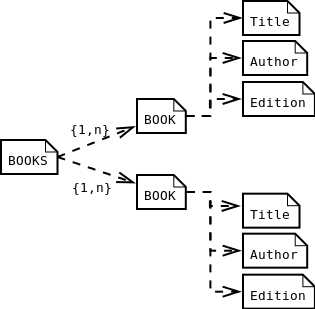
\includegraphics[scale=0.6]{books}
    \caption{Structură arborescentă de date descrisă cu XML}
    \label{fig:imag6}
\end{figure}

\subsection{Structura XML a datelor transmise dinspre server spre aplicația client}
\par Atât aplicația server cât și aplicația client au cea mai mare parte din funcționalitate implementată in extensii (sau plug-in-uri). Din acest motiv, doar o porțiune a mesajelor transmise intre client și server este standardizată. Restul mesajului trebuie să fie structurat conform nevoilor fiecărei extensii de funcționalitate în parte.
\par Mesajele transmise cătra clientul mediului de învățare 3D se clasifică in două categorii:
\begin{itemize}
\item Mesaje de eroare (în cazul în care serverul nu reușește să execute cererea clientului).
\item Răspunsuri ale serverului la cererea aplicației client.
\end{itemize}
\textbf{Structura XML a mesajelor de eroare transmise către aplicația client}
\begin{verbatim}
<?xml version="1.0" encoding="UTF-8"?>"
<response>
  <type></type>
  <exception>
     <message> .... </message>
  </exception>
</response>
\end{verbatim}
\textbf{Structura XML a răspusurilor transmise către aplicația client}
\begin{verbatim}
<?xml version="1.0" encoding="UTF-8"?>
<response>
  <type> TIPUL COMENZII</type>
  <name> NUMELE COMENZII </name>  
  <client_plugin> 
     ------  NUMELE PLUG-INULUI CLIENT -----
  </client_plugin>
  <client_plugin_source> 
     ------ SURSA ONLINE PT DESCĂRCAREA PLUG-IN-ULUI CLIENT -----
  </client_plugin_source>
  <raw>
     ------  FRAGMENT XML CONFORM CERINȚELE FIECĂRUI PLUG-IN ------
  </raw>
</response>"
\end{verbatim}

\section{Schema serverului. Diagrama claselor }
\subsection{Modelarea comenzilor primite de server}
\par Clasa \textbf{ServerCommand} este imaginea câmpurilor XML ce descriu registurl comenzilor și plug-in-urilor apelabile dinamic de către server. Această structură descrie o comandă.
\par Rolul clasei \textbf{CommandProcessor\_step1} este de a despărti textul primit de la aplicația client în subcomponente și de a stoca aceste componente in structura interna a unei instanțe a clasei ServerCommand. Clasa \textbf{CommandProcessor} apelează funcțiile celeor două clase amintite anterior pentru a obține textul răspunsului de trimis către aplicația client.

\begin{figure}[h]
    \centering
    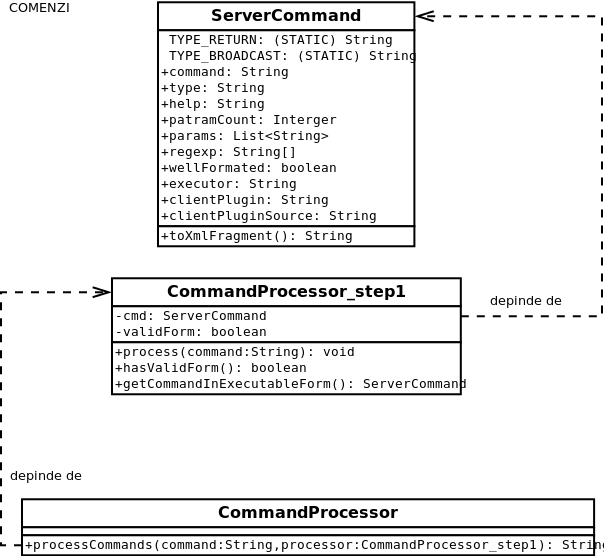
\includegraphics[scale=0.35]{UML-cmd}
    \caption{UML - COMENZI}
    \label{fig:imag7}
\end{figure}